\documentclass[twoside,numberorder]{csbachelor}

%==============================================================
%==============================================================

\usepackage{url}
\usepackage{subfigure}

% 张海:其他引用
\usepackage[hidelinks]{hyperref}
\usepackage{pdfpages}

% 一些全局工具的定义
\DeclareMathOperator*{\argmin}{arg\,min}
\DeclareMathOperator*{\argmax}{arg\,max}

%==============================================================
%==============================================================

\begin{document}

\pagestyle{empty}

%==============================================================
%==============================================================

  % 论文题目:{中文}{英文}
  \zjutitle{标题}
           {Title}
  % 作者:{中文姓名}{英文}{学号}
  \zjuauthor{姓名}{Name}{313XXXXXXXX}
  % 指导教师:{导师中文名}{导师英文名}
  \zjumentor{导师姓名}{Supervisor name}
  % 个人信息:{年级}{专业名称}
  \zjuinfo{2013级}{计算机科学与技术}
  % 学院信息:{学院中文}{学院英文}
  \zjucollege{计算机科学与技术学院}{College of Computer Science and Technology}
  % 日期:{Submitted Date}
  %\zjudate{2017-03-29}

%==============================================================

  \tongjisetup{
  %******************************
  % 注意:
  %   1. 配置里面不要出现空行
  %   2. 不需要的配置信息可以删除
  %******************************
  %
  %=====
  % 秘级
  %=====
  secretlevel={保密},
  secretyear={2},
  %
  %=========
  % 中文信息
  %=========
  % 题目过长可以换行(推荐手动加入换行符,这样就可以控制换行的地方啦)。
  ctitle={同济大学学位论文 \LaTeX{} 模板\\使用示例说明与参考},
  cheadingtitle={同济大学学位论文 \LaTeX{} 模板使用示例说明与参考},    %用于页眉的标题,不要换行
  cauthor={同济人},  
  studentnumber={201804},
  cmajorfirst={工学},
  cmajorsecond={电子控制计算机},
  cdepartment={同济大学Linux用户组},
  csupervisor={陈杰 教授}, 
  % 如果没有副指导老师或者校外指导老师,把{}中内容留空即可,或者直接注释掉。
  cassosupervisor={裴刚 教授~(校外)}, % 副指导老师
  % 日期自动使用当前时间,若需手动指定,按如下方式修改:
  % cdate={\zhdigits{2018}年\zhnumber{11}月},
  % 没有基金的话就注释掉吧。
  cfunds={(本论文由我要努力想办法撑到两行的著名国家杰出青年基金 (No.123456789) 支持)},
  %
  %=========
  % 英文信息
  %=========
  etitle={A Simple Sample of Tongji Thesis\\ Using \tongjithesis{}}, 
  eauthor={Tongji Ren},
  emajorfirst={Gong Xue},
  emajorsecond={DianziControlComputerScience},
  edepartment={TONGJILUG},
  % 日期自动使用当前时间,若需手动指定,按如下方式修改:
  % edate={November,\ 2018},
  efunds={(Supported by the Natural Science Foundation of China for\\ Distinguished Young Scholars, Grant No.123456789)},    
  esupervisor={Prof. Jie Chen},
  eassosupervisor={Prof. Gang Pei (XiaoWai)}
  }

% 定义中英文摘要和关键字
\begin{cabstract}  
  论文的摘要是对论文研究内容和成果的高度概括。摘要应对论文所研究的问题及其研究目
  的进行描述,对研究方法和过程进行简单介绍,对研究成果和所得结论进行概括。摘要应
  具有独立性和自明性,其内容应包含与论文全文同等量的主要信息。使读者即使不阅读全
  文,通过摘要就能了解论文的总体内容和主要成果。

  论文摘要的书写应力求精确、简明。切忌写成对论文书写内容进行提要的形式,尤其要避
  免“第 1 章……;第 2 章……;……”这种或类似的陈述方式。

  本文介绍同济大学论文模板 \tongjithesis{} 的使用方法。本模板符合学校的硕士、
  博士论文格式要求。

  本文的创新点主要有:
  \begin{itemize}
    \item 用例子来解释模板的使用方法;
    \item 用废话来填充无关紧要的部分;
    \item 一边学习摸索一边编写新代码。
  \end{itemize}

  关键词是为了文献标引工作、用以表示全文主要内容信息的单词或术语。关键词不超过 5
  个,每个关键词中间用分号分隔。(模板作者注:关键词分隔符不用考虑,模板会自动处
  理。英文关键词同理。)
\end{cabstract}

\ckeywords{\TeX, \LaTeX, CJK, 模板, 论文}

\begin{eabstract}
   An abstract of a dissertation is a summary and extraction of research work
   and contributions. Included in an abstract should be description of research
   topic and research objective, brief introduction to methodology and research
   process, and summarization of conclusion and contributions of the
   research. An abstract should be characterized by independence and clarity and
   carry identical information with the dissertation. It should be such that the
   general idea and major contributions of the dissertation are conveyed without
   reading the dissertation.

   An abstract should be concise and to the point. It is a misunderstanding to
   make an abstract an outline of the dissertation and words ``the first
   chapter'', ``the second chapter'' and the like should be avoided in the
   abstract.

   Key words are terms used in a dissertation for indexing, reflecting core
   information of the dissertation. An abstract may contain a maximum of 5 key
   words, with semi-colons used in between to separate one another.
\end{eabstract}

\ekeywords{\TeX, \LaTeX, CJK, template, thesis}

  \newpage

\thispagestyle{empty}

{
\setlength{\parindent}{0em}
\renewcommand{\baselinestretch}{2}
\songti\sihao\bfseries

一、 \; 题目: \; \underline{\makebox[24em]{\zjutitlec}}

\vspace{2em}

二、 \; 指导教师对开题报告、外文翻译和中期报告的具体要求:

1. \; 开题报告要求: \; 要求。

2. \; 外文翻译要求: \; 要求。

3. \; 中期报告要求: \; 要求。

\vspace{8cm}
}

{
\songti\xiaosi\bfseries
\begin{flushright}
  指导教师(签名) \; \underline{\hspace{6em}} \\
  年 \qquad 月 \qquad 日
\end{flushright}
}

\ifthenelse{\equal{\zjuside}{T}}{\newpage\mbox{}\thispagestyle{empty}}{}


  \thispagestyle{empty}

{
  \setlength{\parindent}{0em}
  \renewcommand{\baselinestretch}{2}

  {
    \stfangsong\sanhao\bfseries
    \centering
    毕业设计开题报告、外文翻译的考核 \par
  }

  {
    \songti\sihao\bfseries
    导师对开题报告、外文翻译的评语及成绩评定:

    \vspace{10em}

    {
      \renewcommand{\baselinestretch}{1}

      \begin{flushright}

        \begin{tabular}{|c|c|c|c|}
          \hline
          成绩比例 & \parbox[c]{3.6em}{\xiaosi 开题报告 \\ 占(20\%) \vspace{0.25em}} & \parbox[c]{3.6em}{\xiaosi 外文翻译 \\ 占(10\%) \vspace{0.25em}} \\
          \hline
          分值 & & \\
          \hline
        \end{tabular}

        \vspace{2em}

        {
          \songti\xiaosi\bfseries
          导师签名 \; \underline{\hspace{6em}} \\
          年 \qquad 月 \qquad 日 \par
        }
      \end{flushright}
    }
  }

  \vspace{2em}

  {
    \songti\sihao\bfseries
    学院盲审专家对开题报告、外文翻译的评语及成绩评定:

    \vspace{10em}

    {
      \renewcommand{\baselinestretch}{1}

      \begin{flushright}

        \begin{tabular}{|c|c|c|c|}
          \hline
          成绩比例 & \parbox[c]{3.6em}{\xiaosi 开题报告 \\ 占(20\%) \vspace{0.25em}} & \parbox[c]{3.6em}{\xiaosi 外文翻译 \\ 占(10\%) \vspace{0.25em}} \\
          \hline
          分值 & & \\
          \hline
        \end{tabular}

        \vspace{2em}

        {
          \songti\xiaosi\bfseries
          开题报告审核负责人(签名/签章) \; \underline{\hspace{6em}} \par
        }
      \end{flushright}
    }
  }

  \newpage

  {
    \stfangsong\sanhao\bfseries
    \centering
    毕业设计中期报告考核 \par
  }

  {
    \songti\sihao\bfseries
    导师对中期报告的评语及成绩评定:

    \vspace{10em}

    {
      \renewcommand{\baselinestretch}{1}

      \begin{flushright}

        \begin{tabular}{|c|c|c|c|}
          \hline
          成绩比例 & \parbox[c]{3.6em}{\xiaosi 中期报告 \\ 占(10\%) \vspace{0.25em}} \\
          \hline
          分值 & \\
          \hline
        \end{tabular}

        \vspace{2em}

        {
          \songti\xiaosi\bfseries
          导师签名 \; \underline{\hspace{6em}} \\
          年 \qquad 月 \qquad 日 \par
        }
      \end{flushright}
    }
  }
}


  \tableofcontents
  \thispagestyle{toc}
  %\chaptermark{目录}

  \mainmatter

  {
    \pagestyle{kaitibaogao}
    \makeatletter
      \let\ps@plain\ps@kaitibaogao
    \makeatother
    \chapter*{``\zjutitlec'' 开题报告}

\section{项目背景}

\cite{article1}

\section{目标和任务}

\section{可行性分析}

\section{初步技术方案和关键技术考虑}

\section{预期工作结果}

\section{进度计划}

本项目的整体计划如下表所示:

\begin{table}[!htbp]
\centering
\begin{tabular}{|l|l|}
\hline
日期 & 主要工作 \\ \hline
2017-01-01 \textasciitilde\ 2017-02-01 & 开始 \\ \hline
\end{tabular}
\caption{项目进度计划}
\label{table:schedule}
\end{table}

\bibliographystyle{data/gbt7714-2005}
{
\renewcommand{\chapter}[2]{\section*{#2}\addcontentsline{toc}{section}{#2}}
\bibliography{data/kaitibaogao}
}

% 按文章长度需要启用
\ifthenelse{\equal{\zjuside}{T}}{\newpage\mbox{}\thispagestyle{empty}}{}

  }

  {
    \pagestyle{waiwenfanyi}
    \makeatletter
      \let\ps@plain\ps@waiwenfanyi
    \makeatother
    \setcounter{page}{1}

    \renewcommand{\addcontentsline}[3]{}

    {
\renewcommand{\baselinestretch}{1.25}\selectfont

{
  \titleformat{\chapter}[block]{\erhao\songti\bfseries\filcenter}{}{0em}{}{}
  \chapter{本科毕业设计外文翻译}
}

{
  \setlength{\parindent}{0em}

  文献原文:

  A. Bravo, C. Delta. How to translate a sample paper. 2017. \par
}

\vspace{2em}

{
  \renewcommand{\cleardoublepage}{}
  \renewcommand{\clearpage}{}
  \titleformat{\chapter}[block]{\sanhao\songti\bfseries\filcenter}{}{0em}{}{}
  \chapter*{外文翻译标题}
}

\section*{摘要}

\section{前言}

\begin{figure}[!htbp]
\centering

\includegraphics[width=\linewidth,keepaspectratio]{data/waiwenfanyi/placeholder.png}
\caption{Placeholder}
\label{figure:placeholder}
\end{figure}

图~\ref{figure:placeholder}

手动引用~1 {[}1{]}

\section{参考文献}

\begin{itemize}
\item [{[}1{]}] A. Baker, C. Dog. How to make a sample reference. 1938.
\end{itemize}
}

% 按文章长度需要启用
%\ifthenelse{\equal{\zjuside}{T}}{\newpage\mbox{}\thispagestyle{empty}}{}

  }

  \backmatter

  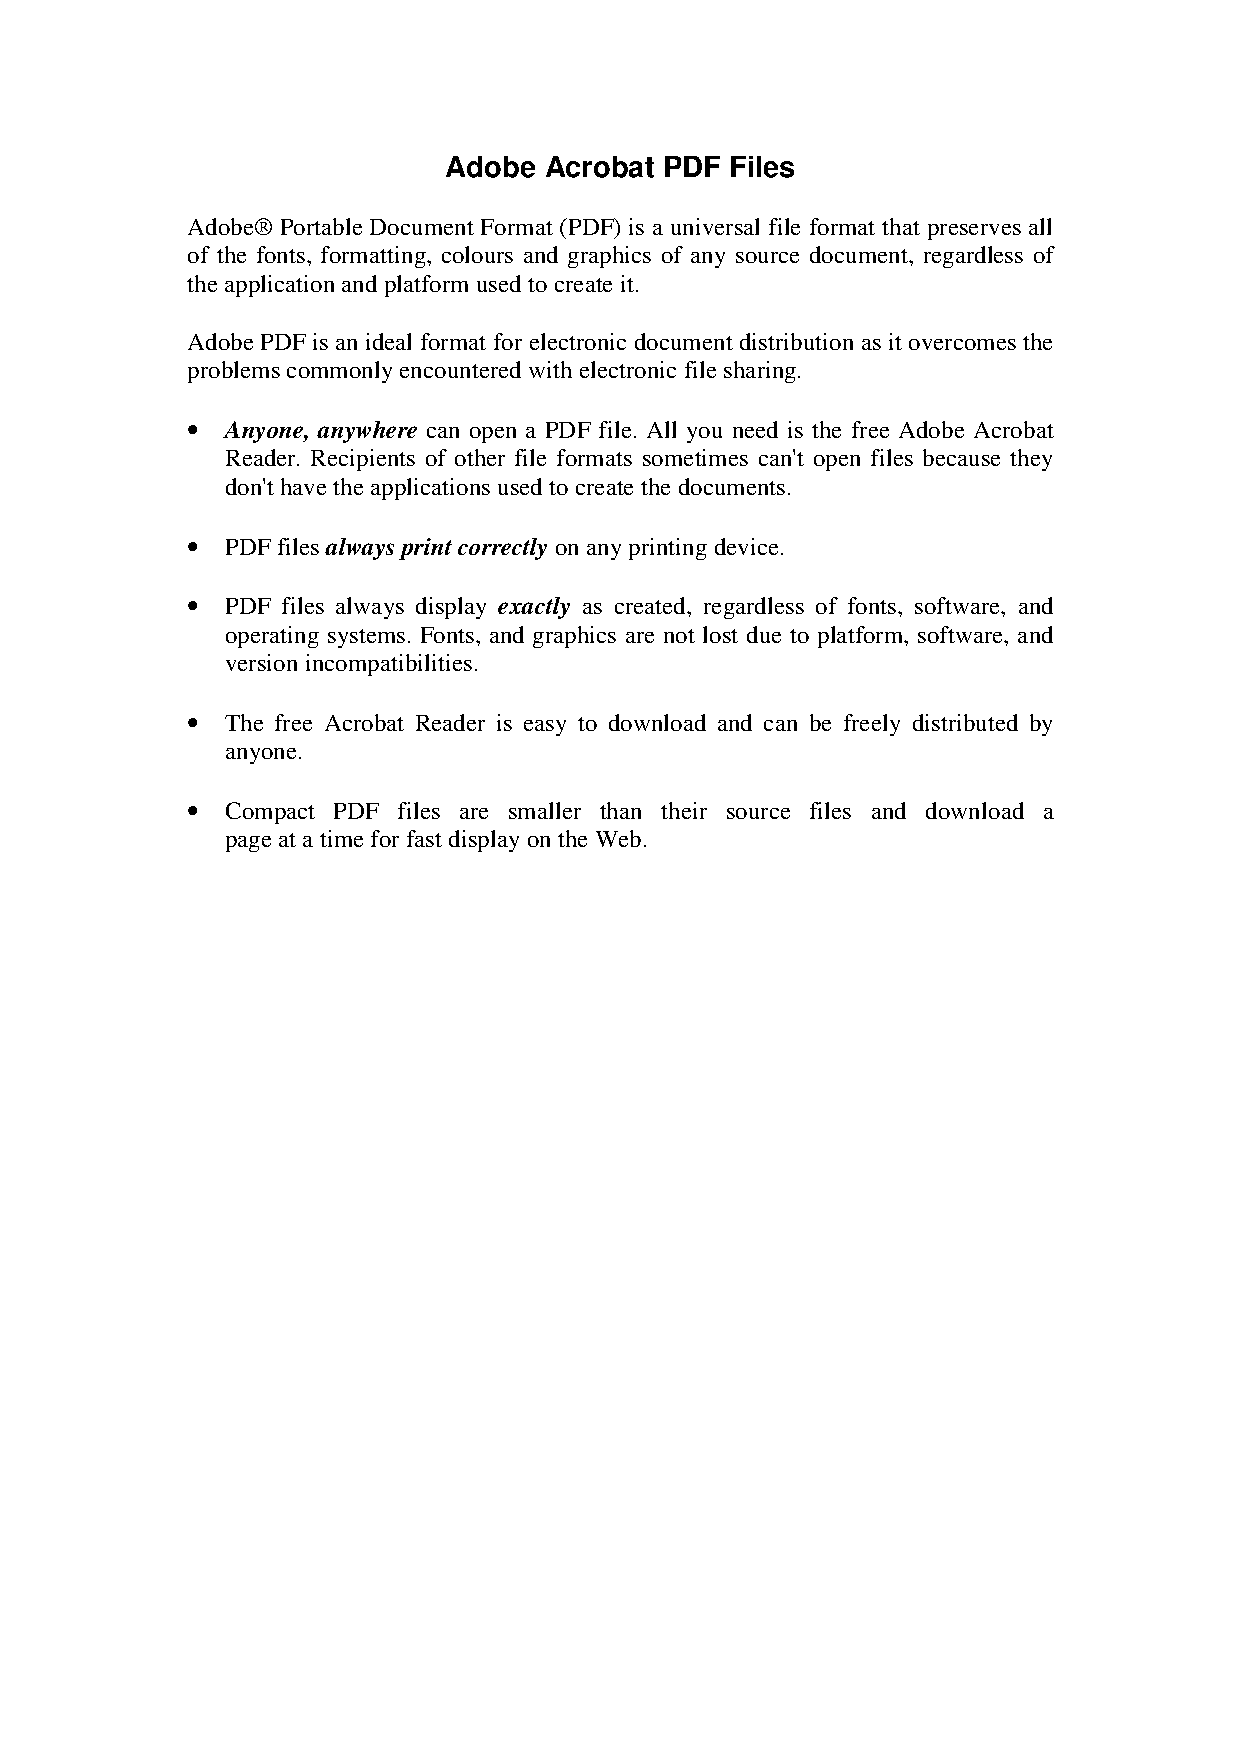
\includepdf[pages=-]{data/waiwenyuanwen.pdf}

\end{document}
